\documentclass{if-beamer}

\title[]{Inner Minkowski Dimension of Products of Fractal Strings}
\subtitle{}
\author{Isaac Ashton, Joseph Ingenito, Peter Tonuzi}
\institute[]{The College of New Jersey}
\date{}
\logo{

\includegraphics[scale=0.10]{tcnj-logotype-400-200.jpg}
}
\subject{MAT 492, Spring 2020} % metadata
\usepackage{animate}
\usepackage{amsmath}
\usepackage{systeme}

\graphicspath{{Images/}}
\usepackage{movie15}
\newcommand{\R}{\mathbb{R}}
\newcommand{\N}{\mathbb{N}}
\newcommand{\SL}{\mathcal{L}}
\newcommand{\Om}{\Omega}
\newcommand{\W}{\mathcal{W}}
\DeclareMathAlphabet{\mathpzc}{OT1}{pzc}{m}{it}
\newcommand{\p}{\mathpzc{p}}
\newcommand{\q}{\mathpzc{q}}
\newcommand{\z}{\mathpzc{z}}
\begin{document}

\begin{frame}
  \titlepage
\end{frame}



\begin{frame}{What We Will Cover}
\text{we're finishing this after our dry run and inevitable cuts}

\end{frame}



\begin{frame}{What is a Fractal String}

\begin{definition}
A {\bf fractal string} $\Om$ is a bounded open subset of the real line.
\end{definition}

\pause
\vspace{.2 in}

$\Omega = \displaystyle\bigcup_{j = 1}^\infty \ell_j$,\qquad $\displaystyle \SL = \text{Vol}_1\left(\Omega\right) = \sum_{j = 1}^\infty \ell_j \implies \lim_{j \to \infty} \ell_j = 0$.

\pause
\vspace{.2 in}

$\ell_1 \geq \ell_2 \geq \ell_3 \geq \cdots \geq 0$

\pause
\vspace{.2 in}

The fractal string we studied the most in particular is the {\bf Cantor String}

\end{frame}



\begin{frame}{Cantor String}
	\begin{center}
		\animategraphics[loop,controls,width=7cm]{10}{Images/CantorStringPNG/CantorStringPNG-}{0}{60}
	\end{center}
\end{frame}



\begin{frame}{Inner-Tubular Neighborhood}

\begin{definition}
{\bf Inner-tubular neighborhood}:\quad $V(\epsilon) = \text{vol}_1\{x \in \Omega\ |\ d(x,\partial\Omega) < \epsilon\}$
\end{definition}

\pause
\vspace{.2 in}

{\bf Counting function}:$\displaystyle \quad N_{\Omega}(x) = \sum_{\ell_j \geq x}1$

\vspace{.2 in}

{\bf More Notation}: $\displaystyle \quad \W_\Om(x) = \sum_{j:\ell_j < x}{\ell_j}$

\vspace{.2 in}

{\bf Now we can write}: $V(\epsilon) = 2\epsilon \cdot N_\Om\left(2\epsilon\right) + \W_\Om\left(2\epsilon\right)$

\end{frame}



\begin{frame}{Cantor String Volume}
	\begin{center}
		\animategraphics[loop,controls,width=7cm]{10}{Images/CantorStringVolumePNG/CantorStringVolumePNG-}{0}{60}
	\end{center}
\end{frame}



\begin{frame}{Inner Minkowski Dimension of a Fractal String}

\begin{definition}
{\bf Dimension of $\Om$}: $D_\Om =\text{inf}\left\{ \alpha \geq 0\ |\ V(\epsilon)=O\left(\epsilon^{1-\alpha}\right) \text{as  } \epsilon \rightarrow 0^{+}\right\}$
\end{definition}

\pause
\vspace{.2 in}

{\bf In other terms}: $D_\Om = \text{the smallest  }\alpha \text{ st } \displaystyle \lim_{\epsilon \to 0^{+}} \frac{V(\epsilon)}{\epsilon^{1-\alpha}}=c, \ c\in \mathbb{R}$

\pause
\vspace{.2 in}

{\bf Cantor String Dimension}: $D_{cs} = \log_3 2$

\end{frame}


%Begin Joe's Section

\begin{frame}{Fractal Lawn}

	\begin{definition}
	A {\bf fractal lawn} $\Om \subset \R^2$ is the Cartesian product of two fractal strings $\Om=\Om_1\times\Om_2$.
	\end{definition}
	
	\pause
	\vspace{0.2 in}

	\[ \displaystyle \SL_1 = \sum_{j \in \N} \ell_j \]
	
	\[ \displaystyle \SL_2 = \sum_{j \in \N} \p_j \]
	\pause
	
	\[ \ell_1 \geq \ell_2 \geq \ell_3 \geq \cdots \geq 0 \], \quad \[ \p_1 \geq \p_2 \geq \p_3 \geq \cdots \geq 0 \]

\end{frame}

\begin{frame}{Cantor Lawn}
	\begin{center}
		\animategraphics[loop,controls,width=7cm]{10}{Images/CantorLawnPNG/CantorLawnPNG-}{0}{60}
	\end{center}
\end{frame}


\begin{frame}{Fractal Lawn Volume I}

{\bf Inner-tubular neighborhood}:\quad $V(\epsilon) = \text{vol}_2\{x \in \Om\ |\ d(x,\partial\Om) < \epsilon\}$
\pause
\vspace{0.2in}

{\bf Useful Definition}:
\begin{itemize}
	\item $\displaystyle \sum_{j = 1}^{N_{\Om_i}(x)}\ell_j=\SL_i - \W_i(x)$
\end{itemize}

\end{frame}


\begin{frame}{Fractal Lawn Volume II}
	\begin{center}
		{\bf Partially Covered Volume Box} \\
		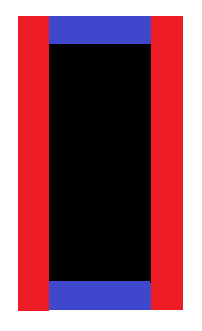
\includegraphics[scale=0.25]{VolumeBox.png}
	\end{center}
	\pause
	\vspace{0.2in}
	
	\begin{itemize}
		\item Partially covered volume
		\begin{itemize}
			\item $\displaystyle V_{partial}(\epsilon)=\textcolor{red}{2\epsilon N_{\Om_1}(2\epsilon)\sum_{j=1}^{N_{\Om_2}(2\epsilon)} \ell_j} + \textcolor{blue}{2\epsilon N_{\Om_2}(2\epsilon)\sum_{j=1}^{N_{\Om_1}(2\epsilon)} (\p_j - 2\epsilon)}$
		\end{itemize}
		\pause
		
		\item Fully covered volume
		\begin{itemize}
			\item $\displaystyle V_{full}(\epsilon)=\SL_1 \W_2(2\epsilon) + \SL_2 \W_1(2\epsilon)$
		\end{itemize}
		\pause
		
		\item Double counted volume
		\begin{itemize}
			\item $V_{double}(\epsilon)=\W_1(2\epsilon) \W_2(2\epsilon)$
		\end{itemize}
	\end{itemize}
	
\end{frame}

\begin{frame}{Fractal Lawn Volume III}

$V(\epsilon)=V_{partial}(\epsilon) + V_{full}(\epsilon) - V_{double}(\epsilon)$
\pause
\vspace{0.2in}

	\begin{align*}
	V(\epsilon)&=2\epsilon \cdot N_{\Om_1}(2\epsilon) \cdot \left(\sum_{j=1}^{N_{\Om_2}(2\epsilon)} \p_j \right) + 2\epsilon \cdot N_{\Om_2}(2\epsilon) \cdot \left(\sum_{j=1}^{N_{\Om_1}(2\epsilon)} (\ell_j - 2\epsilon) \right) + \\
	 &\SL_1 \W_2(2\epsilon) + \SL_2 \W_1(2\epsilon) - \W_1(2\epsilon) \W_2(2\epsilon) \\ \\
	&= 2\epsilon \cdot N_{\Om_1} \cdot (\SL_2 - \W_2) + 2\epsilon \cdot N_{\Om_2} \cdot \left( \SL_1 - \W_1 - 2\epsilon \cdot N_{\Om_1} \right) + \\
	 &\SL_1 \W_2 + \SL_2 \W_1 - \W_1 \W_2 
	\end{align*}
\end{frame}

\begin{frame}{Fractal Lawn Volume IV}
	\begin{center}
		\begin{align*}
		V(\epsilon) &= \SL_1 \cdot (2\epsilon \cdot N_{\Om_2} + \W_2) + \SL_2 \cdot (2\epsilon \cdot N_{\Om_1} + \W_1) - \\
		&(2\epsilon \cdot N_{\Om_1} + \W_1) \cdot (2\epsilon \cdot N_{\Om_2} + \W_2) \\ \\
		&= \SL_1 \cdot \textcolor{blue}{(2\epsilon \cdot N_{\Om_2} + \W_2) }+ \SL_2 \cdot \textcolor{red}{(2\epsilon \cdot N_{\Om_1} + \W_1)} - \\
		&\textcolor{red}{(2\epsilon \cdot N_{\Om_1} + \W_1)} \cdot \textcolor{blue}{(2\epsilon \cdot N_{\Om_2} + \W_2)} \\ \\
		&= \SL_1 \textcolor{blue}{V_2} + \SL_2 \textcolor{red}{V_1} - \textcolor{red}{V_1} \textcolor{blue}{V_2}
		\end{align*}
	\end{center}
\end{frame}

\begin{frame}{Cantor Lawn Volume}
	\begin{center}
		\animategraphics[loop,controls,width=7cm]{10}{Images/CantorLawnVolumePNG/CantorLawnVolumePNG-}{0}{60}
	\end{center}
\end{frame}

\begin{frame}{Dimension of Fractal Lawn I}

\begin{definition}
	The {\bf Dimension} $D_{\Om} = \inf\{\alpha \geq 0\ |\ V(\epsilon) = O(\epsilon^{2 - \alpha})\text{ as }\epsilon \to 0^+\}$
\end{definition}
\pause
\begin{itemize}
	\item Since $\Om \subset \R^2$, V is required to remain bounded by $\epsilon^{2-\alpha} \text{ as }\epsilon \to 0^+ $ rather than the 1D case   
\end{itemize}
\pause
\vspace{0.2in}

	\[ V(\epsilon) &= \SL_1 V_2 + \SL_2 V_1 - V_1 V_2 \]
	\pause
	
	\[ \lim_{\epsilon \to 0^+} V(\epsilon) &= O(\epsilon^{1-D_{\Om_2}}) + O(\epsilon^{1-D_{\Om_1}}) + O(\epsilon^{2-(D_{\Om_1} + D_{\Om_2})})  \]
	
\end{frame}

\begin{frame}{Dimension of Fractal Lawn II}

$\lim_{\epsilon \to 0^+} \frac{V(\epsilon)}{\epsilon^{2-\alpha}} = O(\epsilon^{\alpha - (1+D_{\Om_2})}) + O(\epsilon^{\alpha - (1+D_{\Om_1})}) + O(\epsilon^{\alpha - (D_{\Om_1} + D_{\Om_2})})$
\pause

\[ 
\systeme*{\alpha - (1 + D_{\Om_1}) \geq 0, \alpha - (1 + D_{\Om_2}) \geq 0, \alpha - (D_{\Om_1} + D_{\Om_2}) \geq 0}
\]
\pause

\[ 
D_{\Om} = \text{max} \{ (1 + D_{\Om_1}), (1 + D_{\Om_2}) \}
\]

\end{frame}

\begin{frame}{Dimension of the Cantor Lawn I}

What is the dimension of the Cantor Lawn? \\
\pause
\begin{itemize}
\item Apply the volume formula for a {\bf fractal lawn} to the Cartesian product of 2 Cantor Strings.
\pause 

\item $\Om^2 = \Om \times \Om $
	\pause
	\begin{itemize}
	\item $\Om_1 = \Om_2 $
	\end{itemize}
\pause

\item $D_{\Om^2} = 1 + D_{\Om} = \log_3 2 $
\end{itemize}
\pause

\begin{align*}
V(\epsilon)_{\Om^2} &= \SL V(\epsilon)_{\Om} + \SL V(\epsilon)_{\Om} - V(\epsilon)_{\Om} \cdot V(\epsilon)_{\Om} \\
&= 2 \SL V(\epsilon)_{\Om} - (V(\epsilon)_{\Om})^2
\end{align*}

\end{frame}

\begin{frame}{Dimension of the Cantor Lawn II}
	Let $t = \{-log_3 (2\epsilon)\}$ be defined as the fractional portion of $-log_3 (2\epsilon)$ 
	\begin{align*}
		V_{\Om^2}(\epsilon) &= (2\epsilon)^{1 - log_3 2} \left( 2\left(\frac{1}{2}\right)^t + 2\left(\frac{3}{2}\right)^t \right) + (2\epsilon)^{2- log_3 2} \left( 2\left(\frac{3}{2}\right)^t + 2\left(\frac{1}{2}\right)^t \right) \\
		& - (2\epsilon)^{2- log_3 4} \left( 2\left(\frac{3}{4}\right)^t + \left(\frac{1}{4}\right)^t + \left(\frac{9}{4}\right)^t \right) - (4\epsilon + 4\epsilon^2)
	\end{align*}
	\pause
	
\end{frame}

\begin{frame}{Dimension of the Cantor Lawn III}
\[ 
\systeme*{1- log_3 2 - (2 - \alpha) \geq 0, 2- log_3 2 - (2 - \alpha) \geq 0, 2- log_3 4 - (2 - \alpha) \geq 0}
\]
\pause

\[ 
D_{\Om} = \text{max} \{ (1 + log_3 2), log_3 4 \}
\]
\pause

\[ 
D_{\Om} = 1 + log_3 2
\]
\end{frame}

\begin{frame}{Dimension of the Cantor Lawn IV}
	\begin{center}
		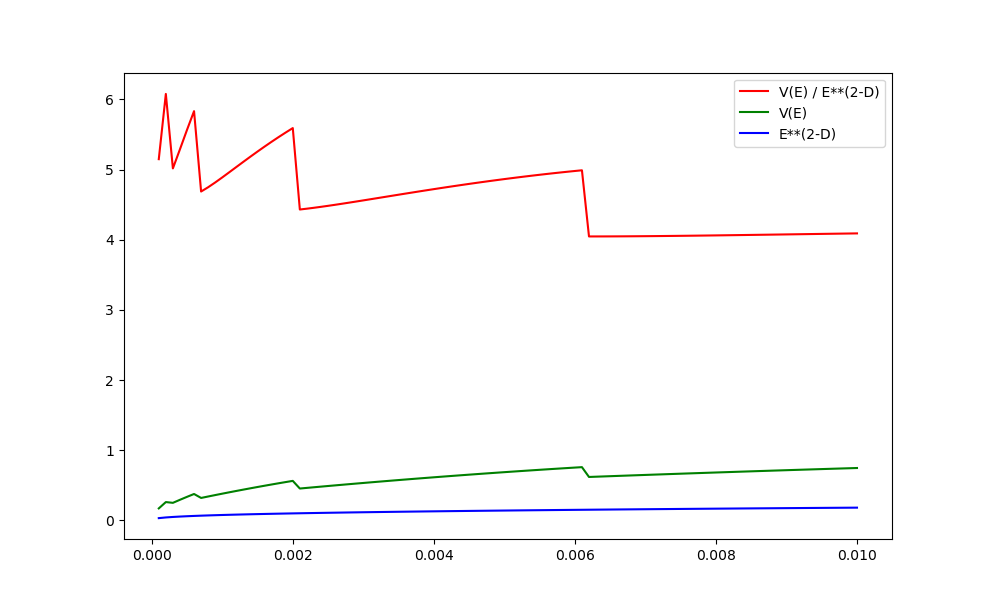
\includegraphics[scale=0.40]{CantorLawnVolumesPlot.png}
	\end{center}
\end{frame}

\begin{frame}{Dimension of the Cantor Lawn V}
	\begin{center}
		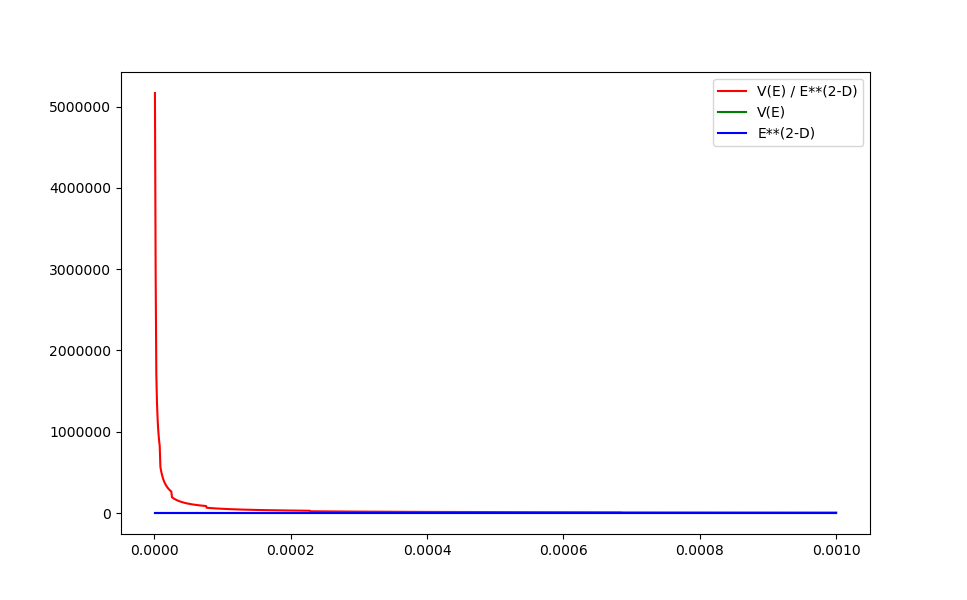
\includegraphics[scale=0.40]{CantorLawnVolumePlot_Alpha-1.png}
	\end{center}
\end{frame}

%begin Peter's part
\begin{frame}{3 Dimensional Fractal Objects}

        \begin{figure}
            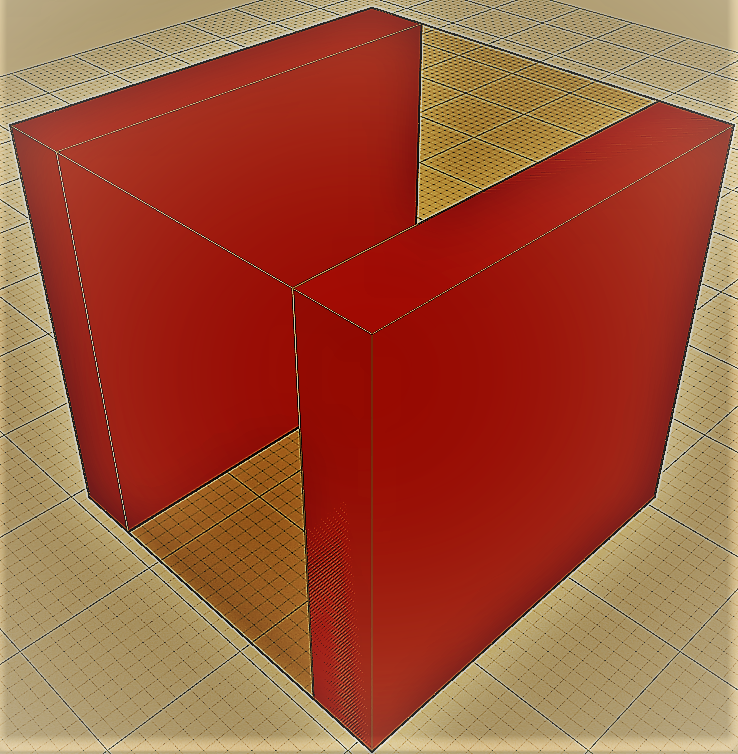
\includegraphics[height=2cm,width=2cm]{3dfractal_1.png}
            \hfill
            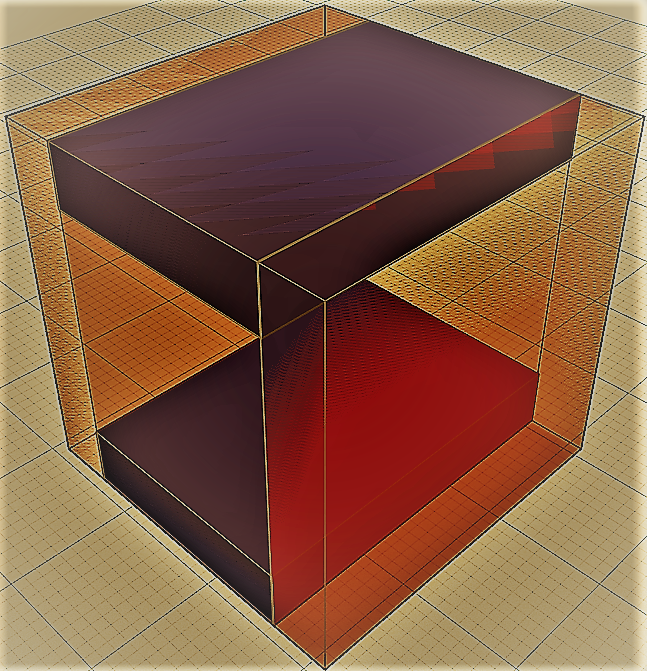
\includegraphics[height=2cm,width=2cm]{3dfractal_2.png}
            \hfill
            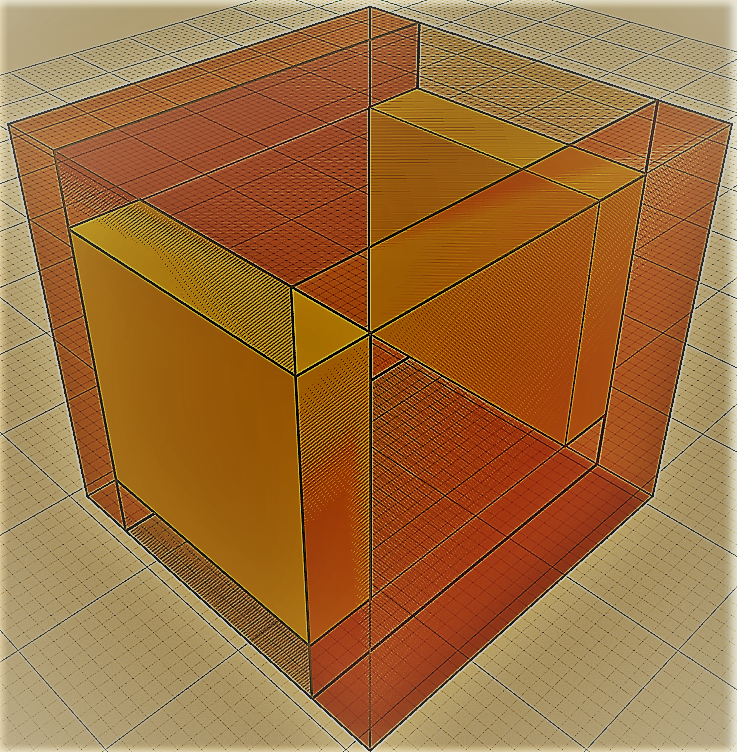
\includegraphics[height=2cm,width=2cm]{3dfractal_3.png}
            \hfill
            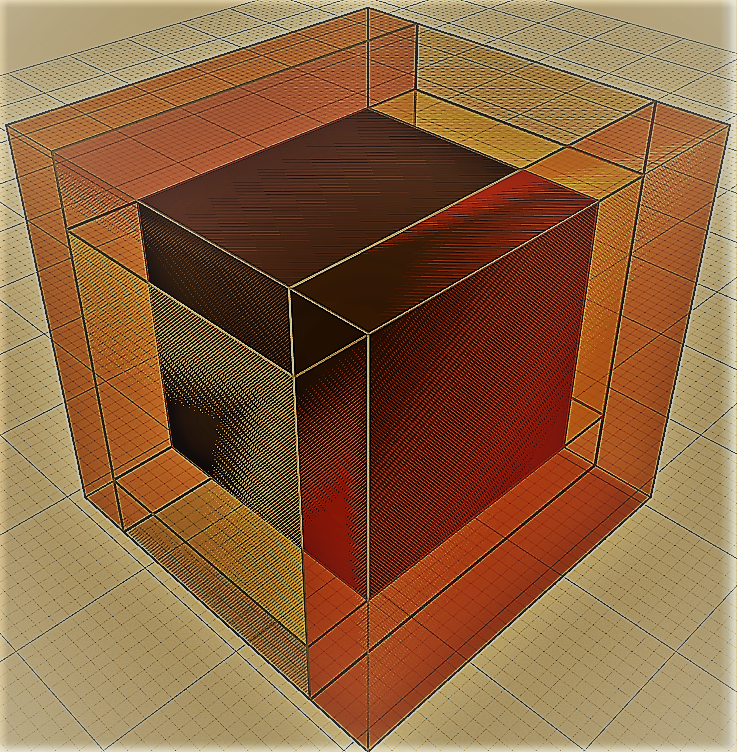
\includegraphics[height=2cm,width=2cm]{3dfractal_4.png}
            \hfill
            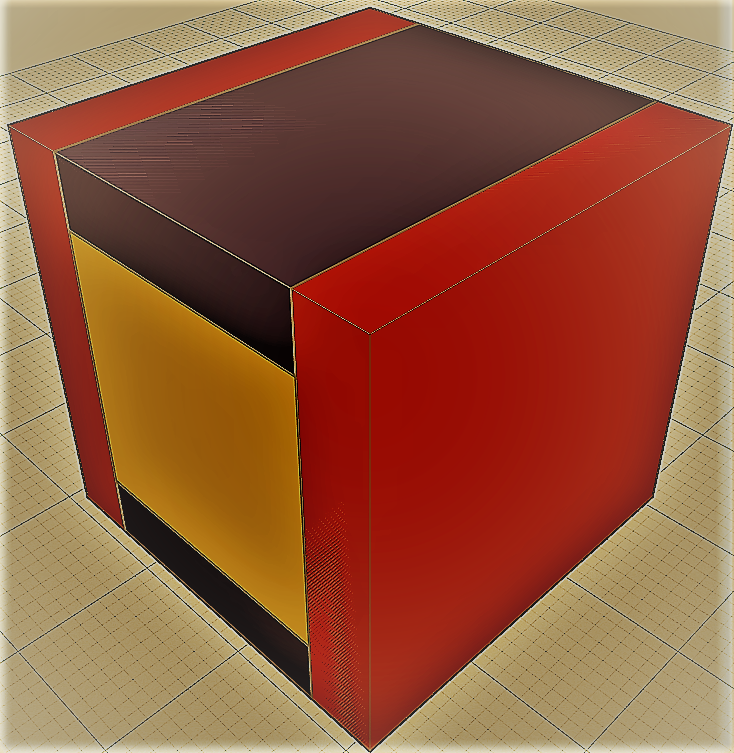
\includegraphics[height=2cm,width=2cm]{3dfractal_5}
        \end{figure}
        
        \begin{align*}
V(\epsilon) &= \textcolor{red}{2\epsilon\cdot N_{\Omega_1}(2\epsilon) \cdot \left( \sum\nolimits_{j=1}^{{N_{\Omega_2}}(2\epsilon)}\p_j \right) \cdot \left( \sum\nolimits_{j=1}^{{N_{\Omega_3}}(2\epsilon)}\q_j \right)} +\\
 &\textcolor{blue}{2\epsilon\cdot N_{\Omega_2}(2\epsilon) \cdot \left( \sum\nolimits_{j=1}^{{N_{\Omega_1}}(2\epsilon)}\ell_j - 2\epsilon \right) \cdot \left( \sum\nolimits_{j=1}^{{N_{\Omega_3}}(2\epsilon)}\q_j \right)} + \\
&\textcolor{yellow}{2\epsilon\cdot N_{\Omega_3}(2\epsilon) \cdot \left( \sum\nolimits_{j=1}^{{N_{\Omega_2}}(2\epsilon)}\p_j - 2\epsilon \right) \cdot \left( \sum\nolimits_{j=1}^{{N_{\Omega_1}}(2\epsilon)}\ell_j - 2\epsilon \right)} + \\
&\W_1\SL_2\SL_3 + \SL_1\W_2\SL_3 + \SL_1\SL_2\W_3 - \SL_1\W_2\W_3 - \W_1\SL_2\W_3 - \\
&\W_1\W_2\SL_3 + \W_1\W_2\W_3 
	\end{align*}
	
\end{frame}

\begin{frame}{3 Dimensional Fractal Volume}
$V(\epsilon) = 2\epsilon \cdot N_{\Omega_1}\cdot(\SL_2-\W_3)\cdot(\SL_3-\W_3) + 2\epsilon \cdot N_{\Omega_2}\cdot(\SL_1-\W_1-2\epsilon\cdot N_{\Omega_1})\cdot(\SL_3-\W_3) + 2\epsilon \cdot N_{\Omega_3}\cdot(\SL_2-\W_2-2\epsilon\cdot N_{\Omega_2})\cdot(\SL_1-\W_1-2\epsilon\cdot N_{\Omega_1}) + \W_1\SL_2\SL_3 + \SL_1\W_2\SL_3 + \SL_1\SL_2\W_3 - \SL_1\W_2\W_3 - \W_1\SL_2\W_3 - \W_1\W_2\SL_3 + \W_1\W_2\W_3$

\pause
\vspace{.2in}

$V(\epsilon) = \SL_1\SL_2V_3(\epsilon) + \SL_1V_2(\epsilon)\SL_3 + V_1(\epsilon)\SL_2\SL_3 - V_1(\epsilon)V_2(\epsilon)\SL_3 - V_1(\epsilon)\SL_2V_3(\epsilon)-\SL_1V_2(\epsilon)V_3(\epsilon) + V_1(\epsilon)V_2(\epsilon)V_3(\epsilon)$
\end{frame}

\begin{frame}{4 Dimensional Fractal Objects}
$V(\epsilon) = 2\epsilon\cdot N_{\Omega_1}(2\epsilon) \cdot \left( \sum_{j=1}^{{N_{\Omega_2}}(2\epsilon)}\p_j \right) \cdot \left( \sum_{j=1}^{{N_{\Omega_3}}(2\epsilon)}\q_j \right) \cdot \left( \sum_{j=1}^{{N_{\Omega_4}}(2\epsilon)}\z_j \right) + 2\epsilon\cdot N_{\Omega_2}(2\epsilon) \cdot \left( \sum_{j=1}^{{N_{\Omega_1}}(2\epsilon)}\ell_j - 2\epsilon \right) \cdot \left( \sum_{j=1}^{{N_{\Omega_3}}(2\epsilon)}\q_j \right) \cdot \left( \sum_{j=1}^{{N_{\Omega_4}}(2\epsilon)}\z_j \right) + 2\epsilon\cdot N_{\Omega_3}(2\epsilon) \cdot \left( \sum_{j=1}^{{N_{\Omega_2}}(2\epsilon)}\p_j - 2\epsilon \right) \cdot \left( \sum_{j=1}^{{N_{\Omega_1}}(2\epsilon)}\ell_j - 2\epsilon \right) \cdot \left( \sum_{j=1}^{{N_{\Omega_4}}(2\epsilon)}\z_j \right) + 2\epsilon\cdot N_{\Omega_4}(2\epsilon) \cdot \left( \sum_{j=1}^{{N_{\Omega_2}}(2\epsilon)}\p_j - 2\epsilon \right) \cdot \left( \sum_{j=1}^{{N_{\Omega_1}}(2\epsilon)}\ell_j - 2\epsilon \right) \cdot \left( \sum_{j=1}^{{N_{\Omega_3}}(2\epsilon)}\q_j - 2\epsilon \right) + \W_1\SL_2\SL_3\SL_4 + \SL_1\W_2\SL_3\SL_4 + \SL_1\SL_2\W_3\SL_4 + \SL_1\SL_2\SL_3\W_4 - \SL_1\SL_2\W_3\W_4 - \SL_1\W_2\SL_3\W_4 - \SL_1\W_2\W_3\SL_4 - \W_1\SL_2\SL_3\W_4 - \W_1\SL_2\W_3\SL_4 - \W_1\W_2\SL_3\SL_4 + \SL_1\W_2\W_3\W_4 + \W_1\SL_2\W_3\W_4 + \W_1\W_2\SL_3\W_4 + \W_1\W_2\W_3\SL_4 - \W_1\W_2\W_3\W_4$
\end{frame}

\begin{frame}{4 Dimensional Volume Formula}
$V^4(\epsilon) = \SL_1\SL_2\SL_3V_4(\epsilon) + \SL_1\SL_2V_3(\epsilon)\SL_4 + \SL_1V_2(\epsilon)\SL_3\SL_4 + V_1(\epsilon)\SL_2\SL_3\SL_4 - V_1(\epsilon)V_2(\epsilon)\SL_3\SL_4 - V_1(\epsilon)\SL_2V_3(\epsilon)\SL_4 - V_1(\epsilon)\SL_2\SL_3V_4(\epsilon) - \SL_1V_2(\epsilon)V_3(\epsilon)\SL_4 - \SL_1V_2(\epsilon)\SL_3V_4(\epsilon) - \SL_1\SL_2V_3(\epsilon)V_4(\epsilon) + V_1(\epsilon)V_2(\epsilon)V_3(\epsilon)\SL_4 + V_1(\epsilon)V_2(\epsilon)\SL_3V_4(\epsilon) + V_1(\epsilon)\SL_2V_3(\epsilon)V_4(\epsilon) + \SL_1V_2(\epsilon)V_3(\epsilon)V_4(\epsilon) -  V_1(\epsilon)V_2(\epsilon)V_3(\epsilon)V_4(\epsilon)$

\pause
\vspace{.2in}

$V^3(\epsilon) = \SL_1\SL_2V_3(\epsilon) + \SL_1V_2(\epsilon)\SL_3 + V_1(\epsilon)\SL_2\SL_3 - V_1(\epsilon)V_2(\epsilon)\SL_3 - V_1(\epsilon)\SL_2V_3(\epsilon)-\SL_1V_2(\epsilon)V_3(\epsilon) + V_1(\epsilon)V_2(\epsilon)V_3(\epsilon)$

\vspace{.2in}

$V^2(\epsilon) = \SL_1V_2(\epsilon) + V_1(\epsilon)\SL_2 - V_1(\epsilon)V_2(\epsilon)$

\end{frame}

\begin{frame}{Algebraic Manipulations}
$V^2(\epsilon) = \SL_1V_2(\epsilon) + V_1(\epsilon)\SL_2 - V_1(\epsilon)V_2(\epsilon)$
$$= (-1)\cdot(V_1(\epsilon)-\SL_1)\cdot(V_2(\epsilon)-\SL_2) + \SL_1\SL_2$$

\pause
\vspace{.2in}

$V^3(\epsilon) = \SL_1\SL_2V_3(\epsilon) + \SL_1V_2(\epsilon)\SL_3 + V_1(\epsilon)\SL_2\SL_3 - V_1(\epsilon)V_2(\epsilon)\SL_3 - V_1(\epsilon)\SL_2V_3(\epsilon)-\SL_1V_2(\epsilon)V_3(\epsilon) + V_1(\epsilon)V_2(\epsilon)V_3(\epsilon)$

$$= (-1)^2\cdot(V_1(\epsilon)-\SL_1)\cdot(V_2(\epsilon)-\SL_2)\cdot(V_3(\epsilon)-\SL_3) + \SL_1\SL_2\SL_3$$

\end{frame}

\begin{frame}{Algebraic Manipulations}
$V^4(\epsilon) = \SL_1\SL_2\SL_3V_4(\epsilon) + \SL_1\SL_2V_3(\epsilon)\SL_4 + \SL_1V_2(\epsilon)\SL_3\SL_4 + V_1(\epsilon)\SL_2\SL_3\SL_4 - V_1(\epsilon)V_2(\epsilon)\SL_3\SL_4 - V_1(\epsilon)\SL_2V_3(\epsilon)\SL_4 - V_1(\epsilon)\SL_2\SL_3V_4(\epsilon) - \SL_1V_2(\epsilon)V_3(\epsilon)\SL_4 - \SL_1V_2(\epsilon)\SL_3V_4(\epsilon) - \SL_1\SL_2V_3(\epsilon)V_4(\epsilon) + V_1(\epsilon)V_2(\epsilon)V_3(\epsilon)\SL_4 + V_1(\epsilon)V_2(\epsilon)\SL_3V_4(\epsilon) + V_1(\epsilon)\SL_2V_3(\epsilon)V_4(\epsilon) + \SL_1V_2(\epsilon)V_3(\epsilon)V_4(\epsilon) -  V_1(\epsilon)V_2(\epsilon)V_3(\epsilon)V_4(\epsilon)$
$$ = (-1)^3\cdot(V_1(\epsilon)-\SL_1)\cdot(V_2(\epsilon)-\SL_2)\cdot(V_3(\epsilon)-\SL_3)\cdot(V_4(\epsilon)-\SL_4) + \SL_1\SL_2\SL_3\SL_4$$
\end{frame}

\begin{frame}{General Volume Formula}

$$V^2(\epsilon)= (-1)\cdot(V_1(\epsilon)-\SL_1)\cdot(V_2(\epsilon)-\SL_2) + \SL_1\SL_2$$

$$ V^3(\epsilon) = (-1)^2\cdot(V_1(\epsilon)-\SL_1)\cdot(V_2(\epsilon)-\SL_2)\cdot(V_3(\epsilon)-\SL_3) + \SL_1\SL_2\SL_3$$

$$ V^4(\epsilon)= (-1)^3\cdot(V_1(\epsilon)-\SL_1)\cdot(V_2(\epsilon)-\SL_2)\cdot(V_3(\epsilon)-\SL_3)\cdot(V_4(\epsilon)-\SL_4) + \SL_1\SL_2\SL_3\SL_4$$

$$V^{n}(\epsilon) =\left[ (-1)^{n-1} \cdot \displaystyle \prod_{k = 1}^{n}(V_k(\epsilon)-\SL_k)\right] +\prod_{k = 1}^{n} \SL_k$$

\end{frame}

\begin{frame}{Future Work}
\begin{itemize}

\item Prove the general volume formula

\item Find a general formula for dimension (based on general volume formula)

\end{itemize}
\end{frame}


\begin{frame}[allowframebreaks]
\frametitle{References}

\begin{thebibliography}{1}

\bibitem{bini2014solving} 
D. A. Bini and L. Robol.
``Solving secular and polynomial equations: A multiprecision algorithm.'' 
\textit{Journal of Computational and Applied Mathematics}
272
(2014),
276--292.

\bibitem{bremner2011lattice} 
M. R. Bremner.
\textit{Lattice Basis Reduction: An Introduction to the LLL Algorithm and its Applications},
Taylor \& Francis, Boca Raton, 2011.

\bibitem{lapidus1991fractal} 
M. L. Lapidus.
``Fractal drum, inverse spectral problems for elliptic operators and a partial resolution of the Weyl-Berry conjecture.'' 
\textit{Transactions of the American Mathematical Society.}
(2)
325
(1991),
465--529.
 
\bibitem{lapidus1993vibrations} 
M. L. Lapidus.
``Vibrations of Fractal Drums, the Riemann Hypothesis, Waves in Fractal Media and the Weyl-Berry Conjecture.'' In \textit{Ordinary and Partial Differential Equations}, edited by B. D. Sleeman and R. J. Jarvis, Vol. IV, Proc. Twelfth Intern. Conf. (Dundee, Scotland, UK, June 1992), Pitman Research Notes in Math. Series 289, pp. 126--209, London: Longman Scientific and Technical, 1993.

\bibitem{lapidus2008in} 
M. L. Lapidus.
\textit{In Search of the Riemann Zeros: Strings, fractal membranes and noncommutative spacetimes}, 
American Mathematical Society, Providence, Rhode Island, 2008.

\bibitem{lapidus2019an} 
M. L. Lapidus.
``An overview of the complex fractal dimensions: From fractal strings to fractal drums, and back,'' \textit{Contemporary Mathematics}, Vol. 731, Amer. Math. Soc., Providence, R.I., 2019, 143--269

\bibitem{lapidus1993the} 
M. L. Lapidus and C. Pomerance.
``The Riemann Zeta-Function and the One-Dimensional Weyl-Berry Conjecture for Fractal Drums,''
\textit{Proc. London Math. Soc.}
(3)
66
(1993),
41--69.

\bibitem{lapidus1995the} 
M. L. Lapidus and H. Maier.
``The Riemann Hypothesis and Inverse Spectral Problems for Fractal Strings.'' \textit{J. London Math. Soc.}
(2)
52
(1995),
15--34.

\bibitem{lapidus2000fractal} 
M. L. Lapidus and M. van Frankenhuijsen.
\textit{Fractal Geometry and Number Theory \textup(Complex dimensions of fractal strings and zeros of zeta functions\textup)},
Birkh\"auser, Boston, 2000.

\bibitem{lapidus2003complex}
M. L. Lapidus and M. van Frankenhuijsen.
``Complex Dimensions of Self-Similar Fractal Strings and Diophantine Approximation,''  
\textit{J. Experimental Math.}
(1)
12
(2003),
41--69. 

\bibitem{lapidus2012fractal} 
M. L. Lapidus and M. van Frankenhuijsen.
\textit{Fractal Geometry, Complex Dimensions and Zeta Functions: Geometry and Spectra of Fractal Strings}, second edition (of the 2006 edition),
Springer Monographs in Mathematics, Springer, New York, 2012.

\bibitem{lapidus2017fractal} 
M. L. Lapidus and G. Radunovi\'c and D. {\u Z}ubrini\'c.
\textit{Fractal Zeta Functions and Fractal Drums: Higher-Dimensional Theory of Complex Dimensions},
Springer Monographs in Mathematics, Springer, New York, 2017.

\bibitem{lenstra1982factoring}
A. K. Lenstra and H. W. Lenstra and L. Lov\'asz.
``Factoring polynomials with rational coefficients,''  
\textit{Mathematische Annalen}
(4)
261
(1982),
515--534. 

\bibitem{schmidt1980diophantine} 
W. M. Schmidt.
\textit{Diophantine Approximation},
Springer, New York, 1980.

\bibitem{serre1973a} 
J.-P. Serre.
\textit{A Course in Arithmetic\textup{, English translation}},
Springer-Verlag, Berlin, 1973.

\bibitem{voskanian2019on} 
E. K. Voskanian.
``On the Quasiperiodic Structure of the Complex Dimensions of Self-Similar Fractal Strings,''
Ph. D. Dissertation, University of California, Riverside, 2019.

\end{thebibliography}

\end{frame}





\end{document}
